\documentclass[fleqn,10pt]{SelfArx} % Document font size and equations flushed left

\usepackage{float}
\usepackage{graphicx}
\usepackage{caption}
\graphicspath{{../figures/}}


\definecolor{color1}{RGB}{0,0,90} % Color of the article title and sections
\definecolor{color2}{RGB}{0,20,20} % Color of the boxes behind the abstract and headings

\JournalInfo{Supplementary Text} % Journal information ``Journal, Vol. XXI, No. 1, 1-5, 2015''
\Archive{ } % Additional notes (e.g. copyright, DOI, review/research article)

\PaperTitle{Supplementary results for: A meta-analysis of computational biology benchmarks reveals publication bias affects on speed and accuracy} % Article title

\Authors{Paul P. Gardner\textsuperscript{1,2}*, James Paterson\textsuperscript{1,2}, Fatemeh Ashari Ghomi\textsuperscript{1,2}, Sinan Uğur Umu\textsuperscript{1,2}, Stephanie McGimpsey\textsuperscript{1,2}} % Authors
\affiliation{\textsuperscript{1}\textit{School of Biological Sciences, University of Canterbury, Christchurch, New Zealand.}} % Author affiliation
\affiliation{\textsuperscript{2}\textit{Biomolecular Interaction Centre and the Bio-Protection Research Centre, University of Canterbury, Christchurch, New Zealand.}}
\affiliation{*\textbf{Corresponding author}: paul.gardner@canterbury.ac.nz} % Corresponding author

\Keywords{computational biology --- accuracy --- benchmarks --- meta-analysis --- software development} % Keywords - if you don't want any simply remove all the text between the curly brackets
\newcommand{\keywordname}{Keywords} % Defines the keywords heading name

%----------------------------------------------------------------------------------------
%	ABSTRACT
%----------------------------------------------------------------------------------------

\Abstract{.}

\begin{document}

\flushbottom % Makes all text pages the same height
\maketitle % Print the title and abstract box
%\tableofcontents % Print the contents section

\thispagestyle{empty} % Removes page numbering from the first page

%----------------------------------------------------------------------------------------
%	ARTICLE CONTENTS
%----------------------------------------------------------------------------------------

\section*{Introduction} % The \section*{} command stops section numbering


XXXX


\clearpage
\newpage

\onecolumn

\begin{figure}[H]
\centering
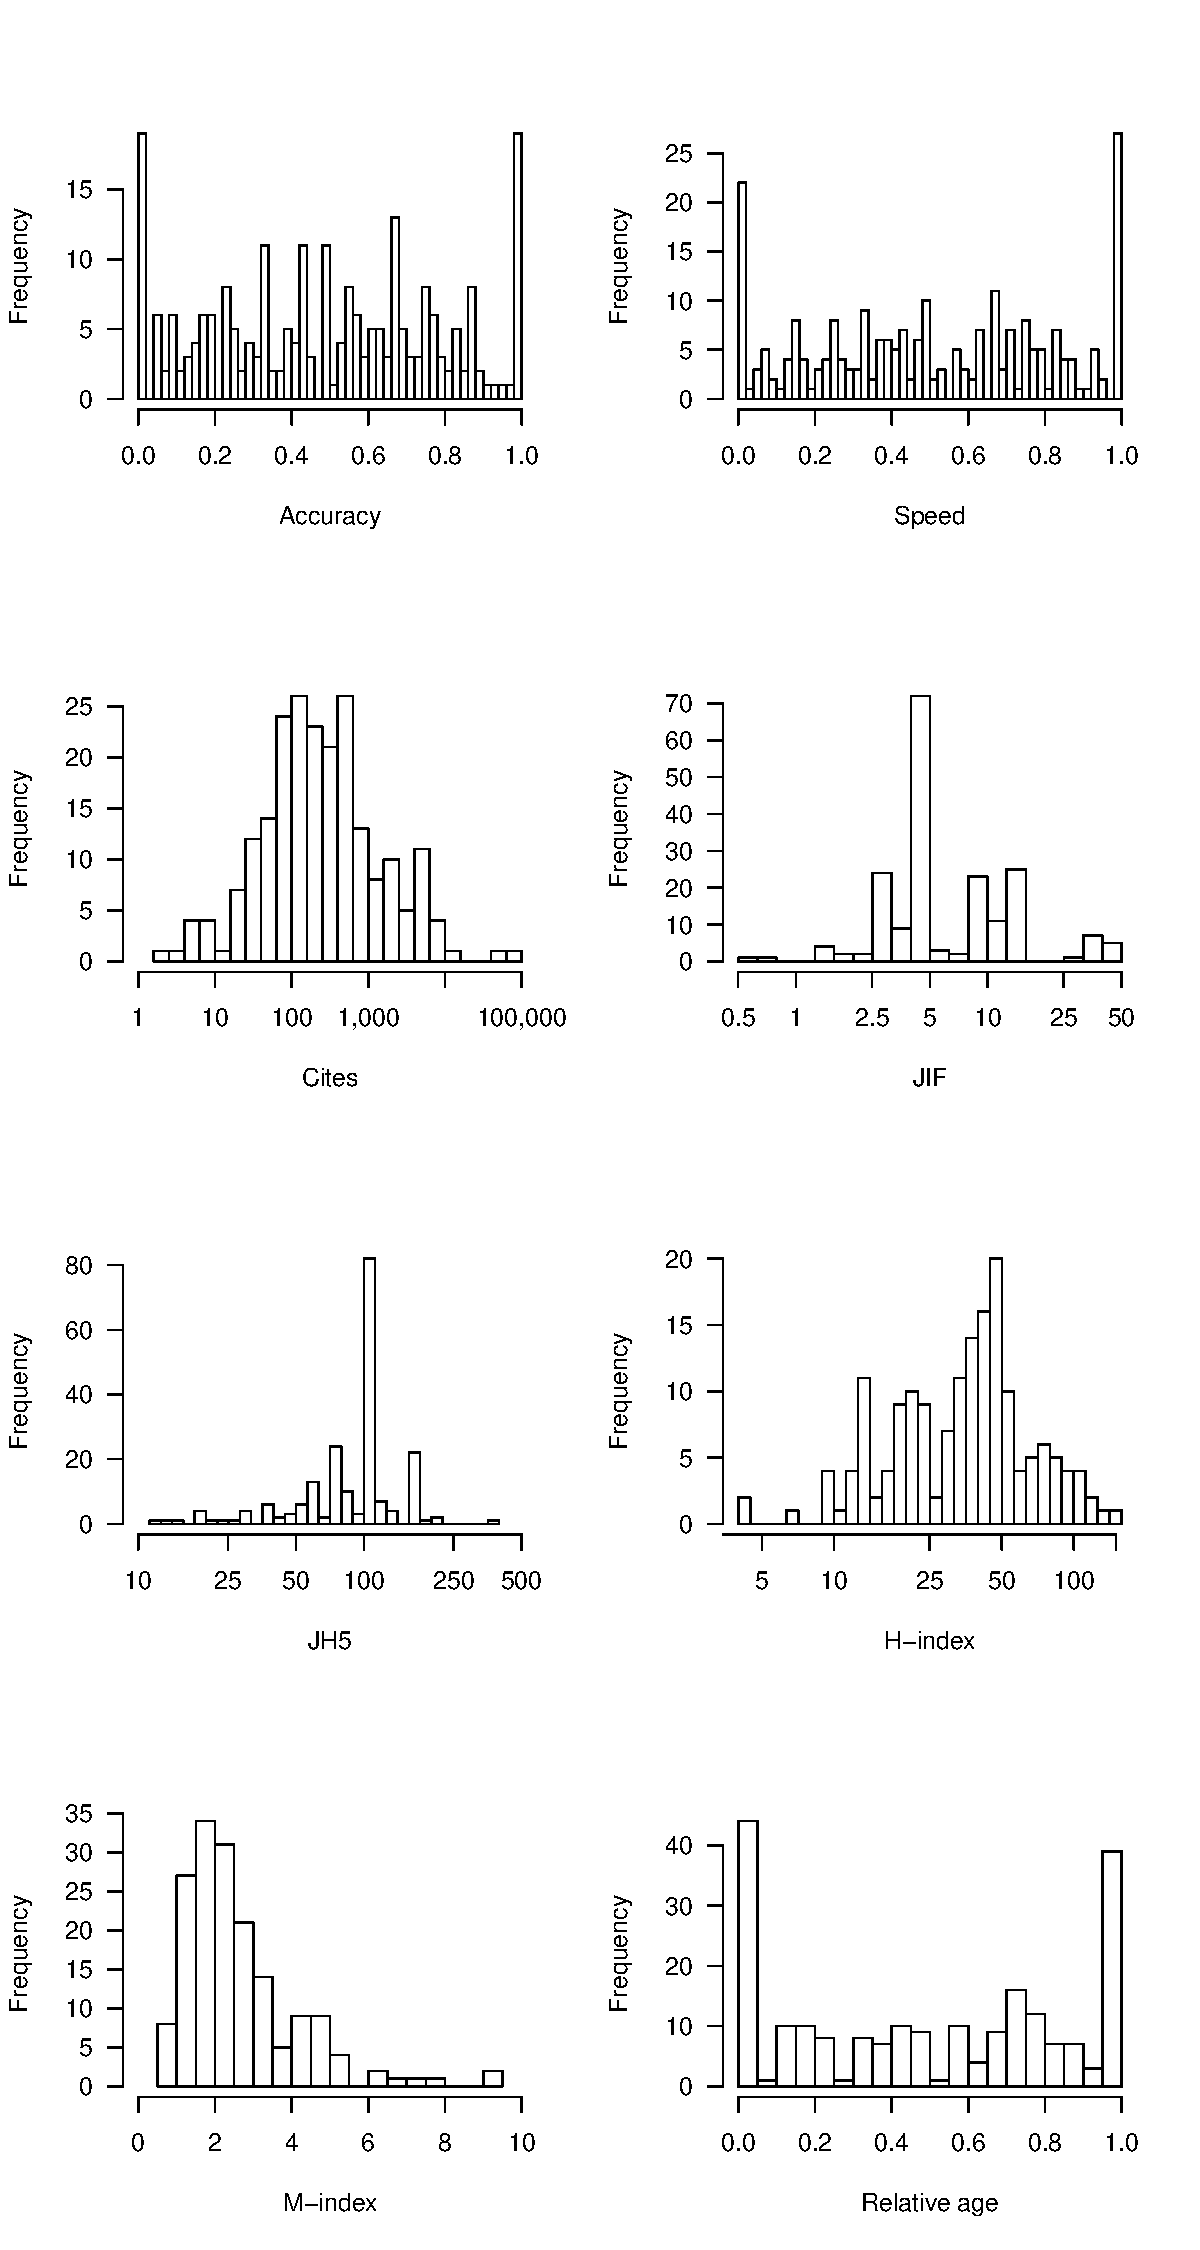
\includegraphics[width=0.55\textwidth]{supplementary-figures-small.pdf}
\caption{The distributions for the metrics used in this study. These
are, reading from left to right, top to bottom: Accuracy -- the mean
normalised accuracy rank for each benchmarked method; Speed -- the
mean normalised speed rank for each benchmarked method; Cites -- the number of
citations to the most cited manuscript describing a method, data from GoogleScholar;
JIF -- the Journal Impact Factor to the highest impact journal that has published
a manuscript describing a method, data from 2014 Thompson-Reuters Citation Reports;
JH5 -- the Journal H5 index to the highest impact journal that has published
a manuscript describing a method, data from GoogleScholar 2015 Metrics;
H-index -- the H-index for the highest profile corresponding author from the
manuscripts describing a method, data from GoogleScholar User Profiles;
M-index -- the M-index (H-index/(\#years since first publication)) for the
highest profile corresponding author from the manuscripts describing a method,
data from GoogleScholar User Profiles;}
\label{fig:S1}
\end{figure}



\begin{figure}[H]
\centering
\includegraphics[width=0.5\textwidth]{smoothScatter-speed-vs-accuracy.pdf}
\caption{...}
\label{fig:S2}
\end{figure}

\begin{figure}[H]
\centering
\includegraphics[width=0.85\textwidth]{smoothScatters.pdf}
\caption{...}
\label{fig:S3}
\end{figure}



\begin{figure}[H]
\centering
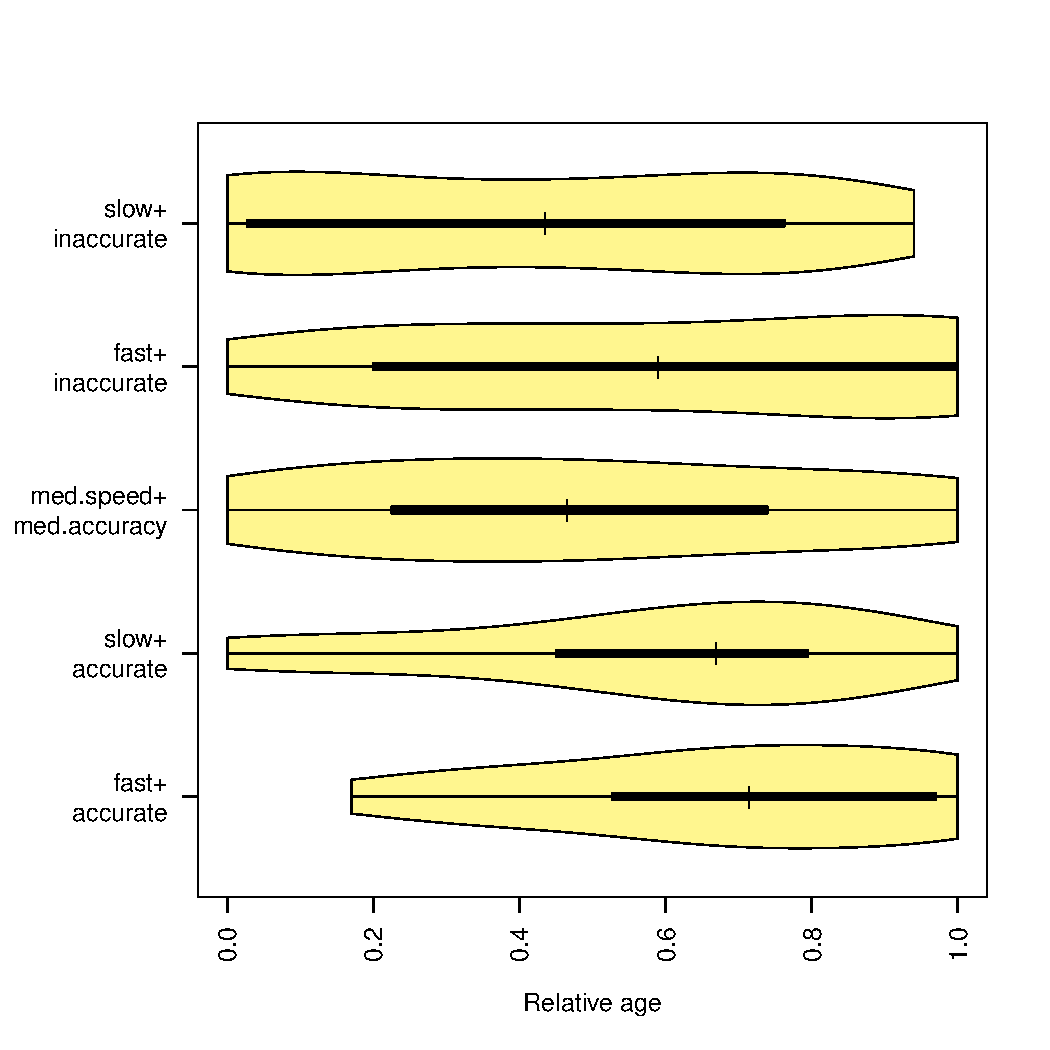
\includegraphics[width=0.45\textwidth]{relAge-speedAcc.pdf}
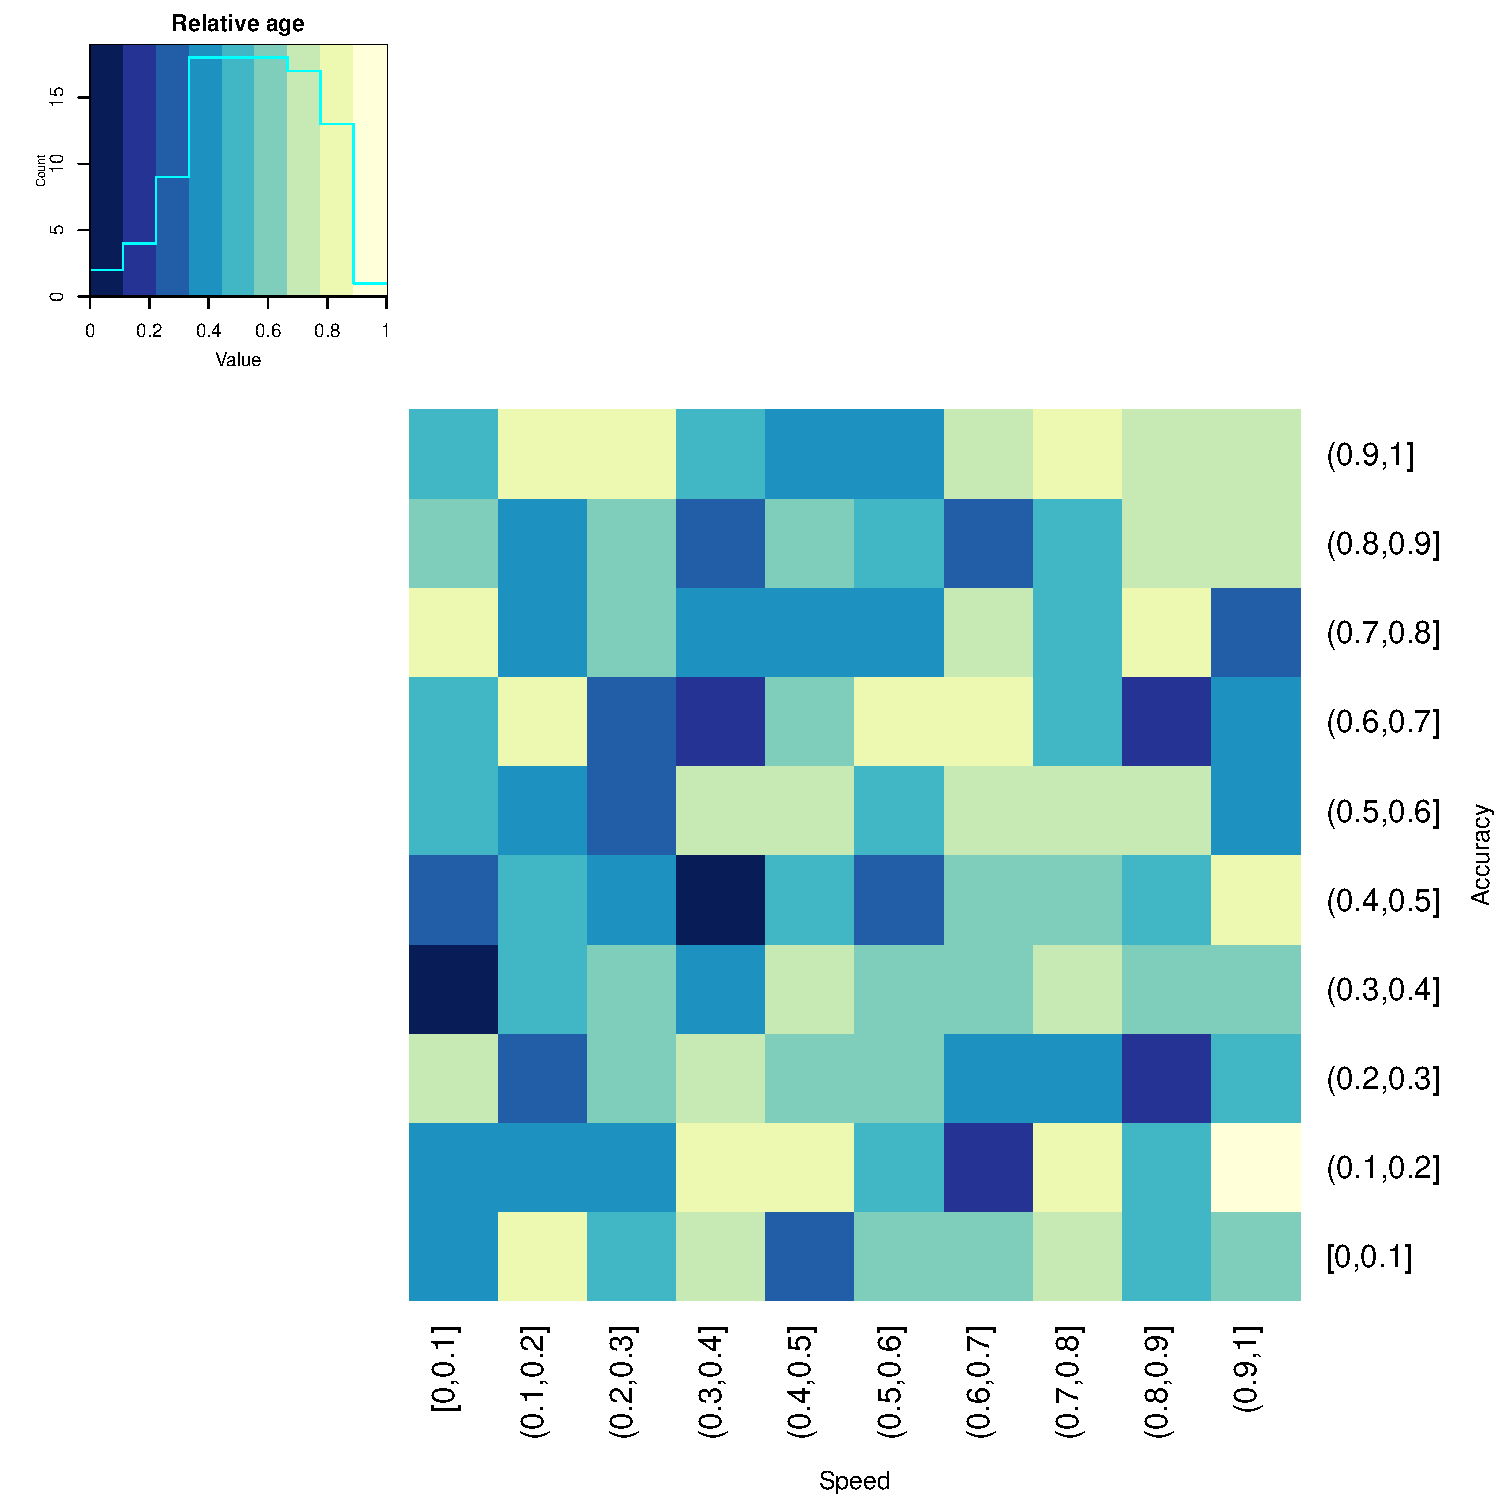
\includegraphics[width=0.45\textwidth]{relAge-SpeedVsAccuracy-heatmap.pdf}\\
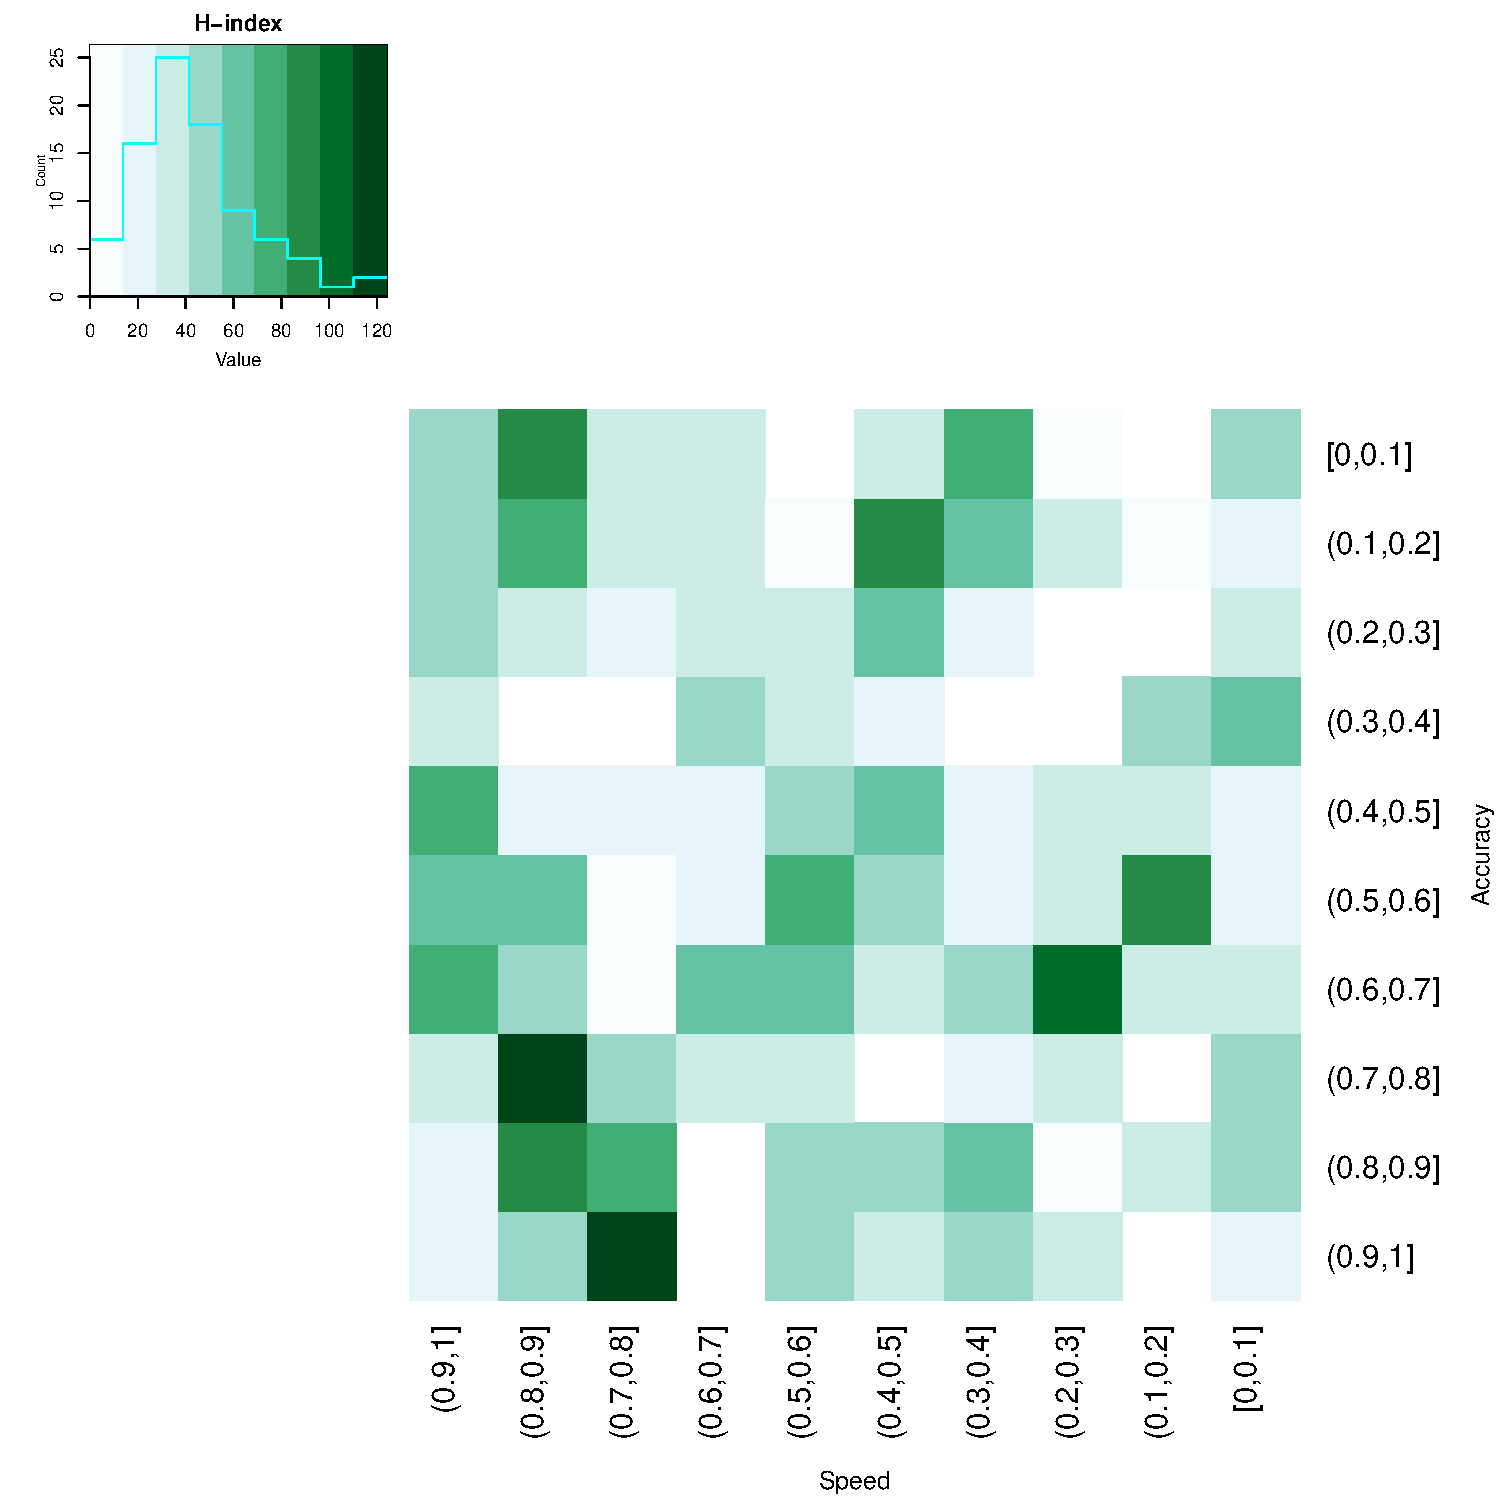
\includegraphics[width=0.45\textwidth]{hindex-SpeedVsAccuracy-heatmap.pdf}
\caption{...}
\label{fig:S4}
\end{figure}


\begin{figure}[H]
\centering
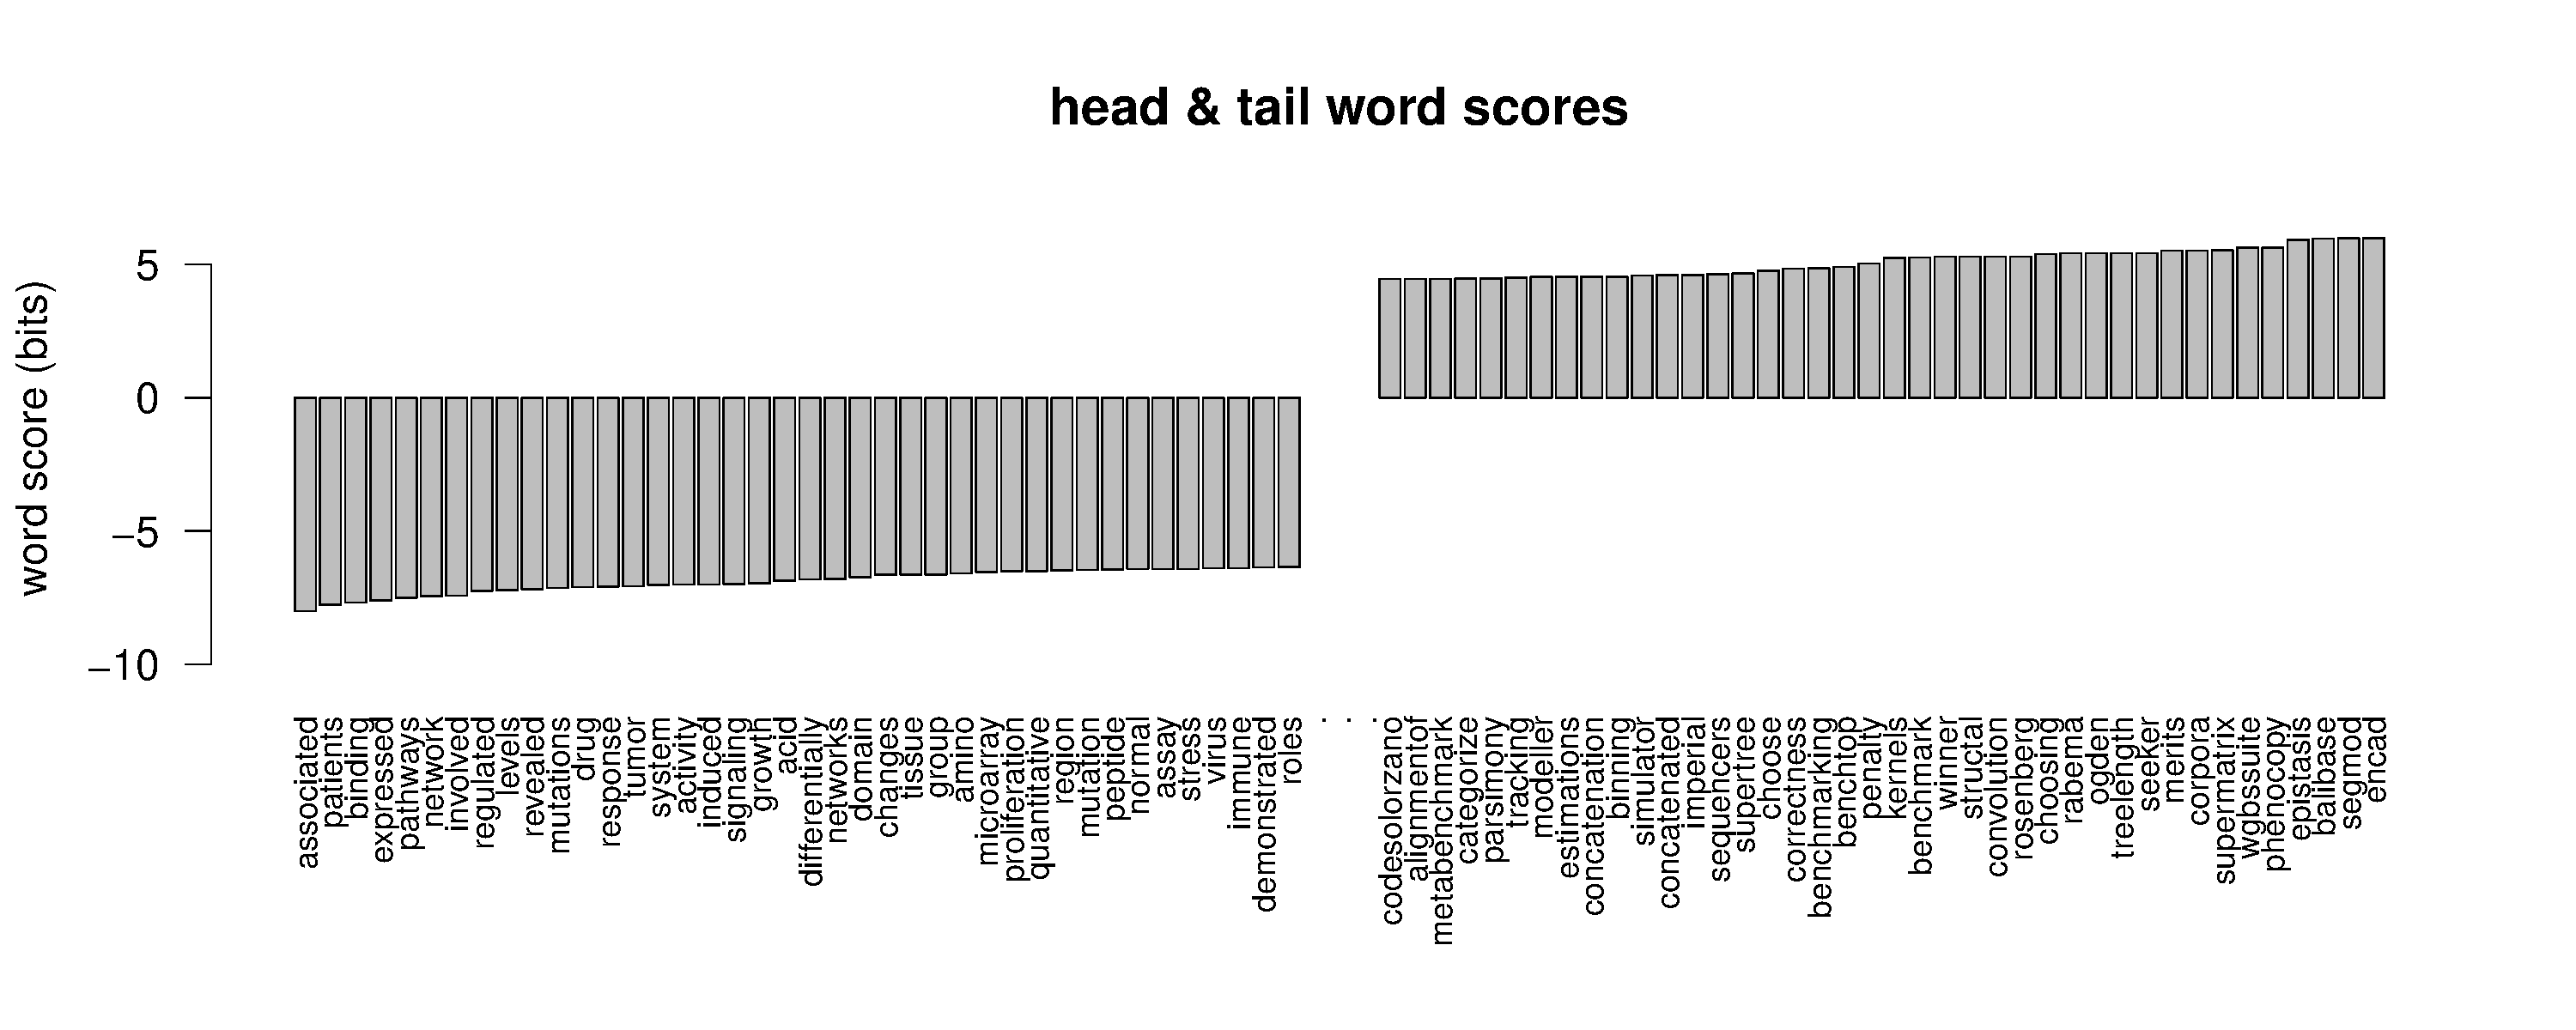
\includegraphics[width=0.85\textwidth]{wordScores.pdf}
\caption{...}
\label{fig:S5}
\end{figure}


%----------------------------------------------------------------------------------------
%	REFERENCE LIST
%----------------------------------------------------------------------------------------
\bibliographystyle{unsrt}
\bibliography{paulall}

\end{document}








